\chapter{Modellierung}
In diesem Kapitel sollen die Anforderungen aus den Interviews praktisch erhoben werden, die Referenzarchitekturen erstellt werden und die konstruierten Referenzarchitekturen folgend auch verglichen werden.
\section{Anforderungserhebung}
Wie in \autoref{theorie:referenzmodellierung} beschrieben, müssen Referenzmodelle einen subjektiven Empfehlungscharakter besitzen, damit sie akzeptiert und wiederverwendet werden. Dafür muss ein Abgleich mit den Anforderungen der Nutzenden geschehen. Um dies zu erreichen, wurden im Anhang transkribierte Interviews (vgl. Anhang~\ref{chap:interview-philipp-22.03.2021}, \ref{chap:interview-peter-24.03.2021}, \ref{chap:interview-ralph-24.03.2021}) durchgeführt. Daraus ergibt sich das in \autoref{abb:TopLevelEchtzeitRA} gezeigte Diagramm, welches die Anforderungen der individuellen Stakeholder an Dekompositiontiefe, Anwendbarkeit und Allgemeingültigkeit darstellt.

\begin{figure}[H]
\centering
\spideroverview
%{P. Arnold}
{5}{3}{3}
%{R. Briegel}
{3}{3}{1}
%{P. Erbacher}
{2}{4}{5}
\caption{Ergebnisse der Interviews}
\label{abb:DimensionenUebersicht}
\end{figure}
Durch die Interviews liessen sich folgende Durchschnitte errechnen: Dekompositionstiefe wurde im Schnitt mit $3,\overline{3}$ bewertet. Die Anwendbarkeit wurde ebenfalls mit $3,\overline{3}$ bewertet. Die Allgemeingültigkeit hingegen hat nur einen Schnitt von $3$. Entsprechend sollten Dekompositionstiefe und Anwendbarkeit priorisiert werden, während die Referenzarchitektur organisationsspezifischer sein darf. 
In den folgenden Referenzarchitekturen wird in mehrere Dekompositionen unterteilt. In der Datenverarbeitungssequenz werden mit Hilfe eines Sequenzdiagramms die Abläufe zur Datenverarbeitung mit dem zu betrachtenden Dienst, ausgehend von \AWSIOT{} Core als Messagebroker gezeigt.
Die Verteilungssicht soll sowohl die Interaktion der Dienste untereinander, als auch grob das durchzuführende Deployment zeigen. Die Bausteinsicht zeigt wichtige Elemente der einzelnen Dienste auf, die konkret untereinander interagieren. So ist die konkrete Untereinheit, die Daten von \AWSIOT{} Core an andere Dienste versendet eine \AWSIOT{} Core Rule, welche aufzuzeigen wäre. \TodoW{Genauere Auswirkungen}

Für die Operations wird vorausgesetzt, dass der \ac{AWS}-native Dienst CloudWatch zur Überwachung eingesetzt wird. 
\begin{figure}[H]
\centering
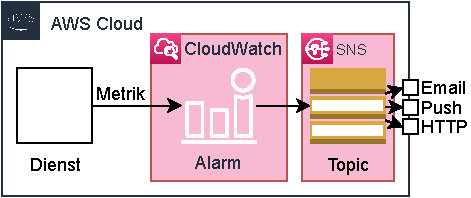
\includegraphics[width=0.66\textwidth]{graphics/CloudWatch-Monitoring}
\caption{CloudWatch Monitoring}
\label{abb:CloudWatchMonitoring}
\end{figure}
CloudWatch erfasst zentralisiert Metriken aller Dienste und löst bei nutzerdefinierten Überschreitungen einen Alarm aus, welcher dann via \ac{SNS} versendet werden kann (siehe \autoref{abb:CloudWatchMonitoring}).



Zusätzlich haben sich folgende Anforderungen ergeben:
\begin{itemize}
\item Anwendbarkeit auf Monitoring (klassische IT) (Anhang \ref{chap:interview-philipp-22.03.2021}, \ref{chap:interview-peter-24.03.2021})
\item Anwendbarkeit auf Sensordaten (\ac{IoT}) (Anhang \ref{chap:interview-philipp-22.03.2021}, \ref{chap:interview-peter-24.03.2021}, \ref{chap:interview-ralph-24.03.2021})
\item Wertschöpfung für den Betrieb wichtig
\item akzeptabel und problemlösend für Domäne
\item Handling von Events, Messwerten und \enquote{Streaming} (Anhang \ref{chap:interview-peter-24.03.2021})
\end{itemize}

% \begin{figure}[H]
% \centering
% 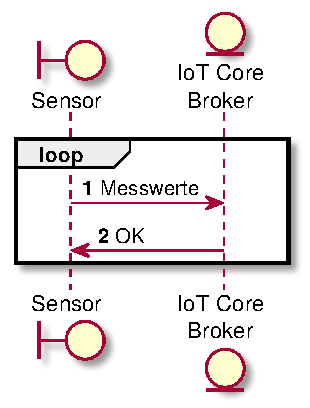
\includegraphics[height=0.3\textheight]{graphics/dateneinspeisung.pdf}
% \caption{Sequenzdiagramm Dateneinspeisung}
% \label{abb:SequenceEinspeisung}
% \end{figure}

Im Folgenden werden die Referenzarchitekturen entworfen und miteinander verglichen, um mögliche Stärken und Einsatzgebiete zu identifizieren.

\section{Echtzeitverarbeitung}
Aufgrund des in \autoref{tab:bewertungsmatrix-echtzeit} durchgeführten Vergleiches, den Kinesis (Data Streams und Analytics) anführte, wird im Folgenden die Referenzarchitektur für die Echtzeitverarbeitung mit Kinesis Data Streams und Analytics entworfen. 

\subsection{Datenverarbeitungssequenz}
In \autoref{abb:SequenceEchtzeitRA} wird die durchlaufene Sequenz für eingehende Daten gezeigt. Nach initialer Übertragung via \ac{MQTT} an \AWSIOT{} Core, folgt die Übertragung in Kinesis Data Streams, welche die Daten gepuffert an Kinesis Data Analytics sendet. 

\begin{figure}[H]
\centering
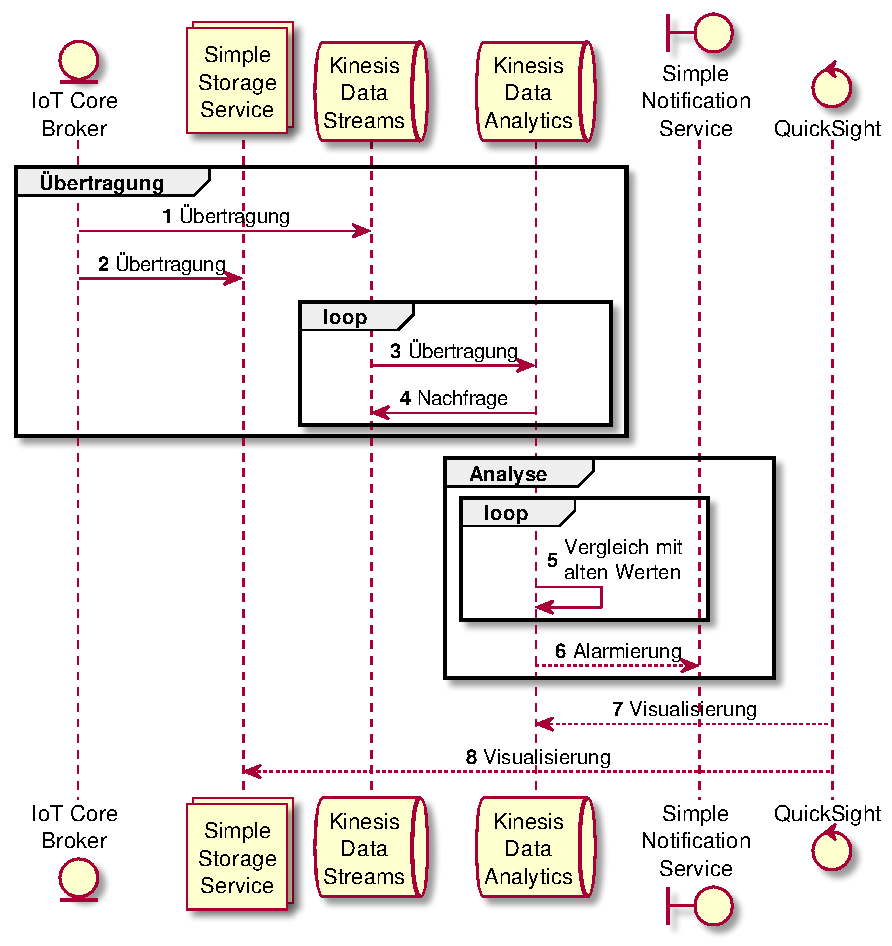
\includegraphics[height=0.66\textheight]{graphics/echtzeit-ra.pdf}
\caption{Sequenzdiagramm Echtzeitreferenzarchitektur}
\label{abb:SequenceEchtzeitRA}
\end{figure}

\subsection{Verteilungssicht}
Folgend ist die Verteilungssicht der Echtzeitreferenzarchitektur gezeigt. Die gestrichelte Linie zu QuickSight ist vorhanden, da der Variationspunkt 3 die konkrete Anwendung variiert.
\begin{figure}[H]
\centering
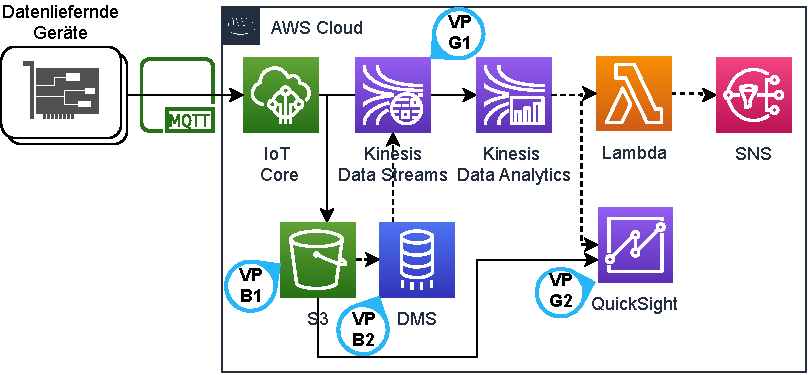
\includegraphics[width=\textwidth]{graphics/Echtzeit-RA-Overview.pdf}
\caption{Top Level View Referenzarchitektur}
\label{abb:TopLevelEchtzeitRA}
\end{figure}
Variationspunkt 1: Rohdaten in \ac{S3} zu speichern kann Sinn machen, um die Daten später noch einmal analysieren zu können. Nimmt man aber die Theorie der Datenhalbwertszeit zur Hilfe, macht es vielleicht Sinn die Daten statdessen maximal 48h in Kinesis zwischenzuspeichern und auf \ac{S3} zu verzichten. Mittels der erweiterten Aufbewahrung $\lbrack$\textit{Data Retention}$\rbrack$ können Analysen mehrfach im Fehlerfall angefordert werden. Da die Preise nach sieben Tagen Aufbewahrung ansteigen und für Aufbewahrung und Abruf doppelt abgerechnet wird, ist zu empfehlen, nach sieben Tagen die Daten zu verwerfen.\footcite[Vgl.][]{AmazonWebServicesInc..o.J.l}

Variationspunkt 2: \ac{DMS} ist in diesem Szenario dafür gedacht, einmal abgelegte Daten in S3 wieder in Kinesis Data Streams einspielen zu können. Je nach Szenario ist dies, wie bei Variationspunkt 1 schon erläutert, nicht notwendig.

Variationspunkt 3: QuickSight als \ac{AWS} native Dashboardlösung ist gut geeignet, um schnell Übersicht in Datenanalysen aus Kinesis Data Analytics zu bekommen. Alternativ können auch andere Visualisierungslösungen wie Tableau eingesetzt werden, welche gegebenenfalls jedoch keinen (vollen) Zugriff auf Kinesis Data Analytics haben. Ein weiterer managed Service, den \ac{AWS} für Dashboards anbietet, ist der Amazon Managed Service for Grafana, welcher das Open Source Visualisierungstool Grafana mit den \ac{AWS} eigenen Metriken integriert.\footcite[Vgl.][]{Dutt.2020} In diesem Fall kann der aus Variationspunkt 1 bekannte \ac{S3} Bucket aufgesetzt werden, um Dashboards über die Rohdaten zu erstellen. 

\subsection{Bausteinsicht}
Folgend ist als weitere Dekomposition die Bausteinsicht gezeigt.
\begin{figure}[H]
\centering
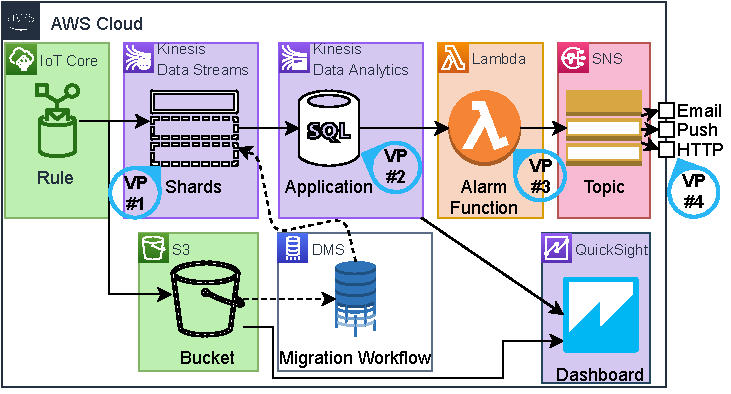
\includegraphics[width=\textwidth]{graphics/Echtzeit-RA-Elements.pdf}
\caption{Interagierende Dienstelemente}
\label{abb:ElementeEchtzeitRA}
\end{figure}
Variationspunkt 1: Die Anzahl an Shards ist essentiell für die Performance von Kinesis Data Streams. Für Workloads mit einem vorhersehbaren Workload ist Anzahl an Shards nach einem Preis/Leistungs Optimum zu ermitteln und zu konfigurieren. Wenn der Workload nicht vorhersehbar ist oder schnell skalieren können soll, sind Alarme im AWS eigenen Monitoring Tool CloudWatch zu erstellen. Im Beispielusecase für die Kostenschätzung ist ein einziger Shard (1MiB/Sekunde, 1000 Nachrichten eingehend) ausreichend. Dies ist bedingt, da Nachrichten mit einer Größe von 1KB, also ca. 1KiB geschrieben werden, bei einem Maximum von 200 pro Sekunde und einem Konsumenten. Es ist besonders auf die \enquote{WriteProvisionedThroughputExceeded} Metrik zu achten, welche bei höheren Werten anzeigt, dass das Hinzufügen von zusätzlichen Shards angebracht wäre. Ebenfalls ist die Metrik \enquote{Incoming Records} zu beachten. Verändert diese sich, deutet das auf einen Fehler im vorgelagerten \AWSIOT{} Core oder in einem Teil der Datenlieferanten hin.

\TodoW{Flink ausbauen ggf. auch in Beschreibung}

Variationspunkt 2: Der \ac{SQL} Programmcode, der in Kinesis Data Analytics läuft ist anzupassen. So sind Verarbeitungsfenster, Attributsnamen und aufgerufene Funktionen nach Anforderung zu ändern. Andernfalls kann auch die Funktionalität zur Ausführung eigenen Codes via Apache Flink in Kinesis Data Analytics genutzt werden (dies erlaubt Ausführung von Java, Scala, Python).

Variationspunkt 3: Aufgrund der Notwendigkeit einer Lambda Funktion, um Alarme zu versenden, kann der Code selbst gestaltet werden. Wichtig ist dabei, dass Kinesis Data Analytics die Zustellung von Datensätzen wiederholt, wenn die Lambdafunktion als Rückgabewert ein Array mit den Ids und dem Status wie folgt zurückgibt: \mintinline[breaklines]{json}{[{"recordId": "<ID>", "result": "DeliveryFailed"}]}.\footcite[Vgl.][]{AmazonWebServicesInc..o.J.ay} Die übermittelten Alarme lassen dabei Möglichkeit zur Anpassung. So kann neben dem Titel der Nachricht auch der eigentliche Inhalt angepasst werden. 

Variationspunkt 4: \ac{SNS} unterstützt mehrere Protokolle für die Übermittlung von Nachrichten. Es können HTTP Webhooks genauso wie mobile Pushbenachrichtigungen oder auch Emails versendet werden. Welches Protokoll mit welchem Verteiler zu wählen ist, muss im \ac{SNS} Topic eingestellt werden. Innerhalb der Cloud Native Solution der SPIRIT/21 hat sich bewährt, den Versand via Email zu nutzen und als Ziel den Email-Verteiler eines Monitoring Teams innerhalb des Tools Microsoft Teams einzustellen. Microsoft Teams zeigt eingegangene Emails an den Emailverteiler dann als Chatnachricht innerhalb des Teams an und benachrichtigt alle Teilnehmenden.

\subsection{Anforderungen}
\begin{itemize}
\item Anwendbarkeit auf Monitoring (IT)\\
Kinesis als System ist gut auf diverseste Zeitseriendaten anwendbar. Problematisch ist das eigene Übertragungsformat, welches von Datenproduzenten verlangt, spezielle Schnittstellen zu implementieren. Der von \ac{AWS} vorgesehene Weg, die Kinesis Producer Library ist in Java geschrieben und bindet eine ausführbare C++ Datei ein.\footcite[Vgl.][]{AmazonWebServicesInc..o.J.bg} Im Einsatz mit Monitoringdaten würde dies erfordern, dass die Daten in einem Standardformat aggregiert und dann mittels eines in Java geschriebenen Programms transformiert werden müsste. Alternativ können noch die \enquote{Kinesis Record Aggregation \& Deaggregation Modules for AWS Lambda} von \ac{AWS} verwendet werden, welche die Daten in das aggregierte, kinesiseigene Format umwandeln.\footnote{Siehe \url{https://github.com/awslabs/kinesis-aggregation}} Diese Module haben Sprachkompatibilität zu Java, JavaScript/Node.js und Python.

\item Anwendbarkeit auf Sensordaten (\ac{IoT})\\
Kinesis ist generalisiert ausgelegt, durch die Integration mit \AWSIOT{} Core wird jedoch die Verarbeitung von \ac{IoT} Daten leicht gemacht. 

\item Wertschöpfung für den Betrieb wichtig\\
\TodoW{Interview}
\item akzeptabel und problemlösend für Domäne\\
\TodoW{ausfüllen}
\item Handling von Events, Messwerten und \enquote{Streaming}\\
Da die Verarbeitungslogik in Kinesis Data Analytics selbst zu schreiben ist, ist die unterschiedliche Behandlung von Events, niedrigfrequenten Messwerten und Streaming implementierungsabhängig. Dabei wäre es zu empfehlen ein Attribut in die übermittelten Nachrichten einzufügen, welches den geanauen Typ der Nachricht definiert und entsprechende Verarbeitungslogiken vereinfacht. Zu diesem Zweck soll das Attribut \mintinline[breaklines]{json}{{"messageType": "<string>"}} dienen. Für Events, die Definitionsgemäß keinen Messwert beinhalten, ist das Attribut mit dem Wert \mintinline[breaklines]{json}{{"messageType": "event"}} zu belegen. Messwerte sollen \mintinline[breaklines]{json}{{"messageType": "meas_low_freq"}} als Wert verwenden. Für hochfrequentes Streaming ist \mintinline[breaklines]{json}{{"messageType": "meas_high_freq"}} zu verwenden.

\item automatisierte operative Entscheidungen

Automatisierte Entscheidungen bzw. Handlungen sind mit Kinesis Data Analytics möglich. So könnte die selbe Lambdafunktion, die für die Alarmierung benutzt wird, auch Aktionen auslösen. Vorstellbar wäre, dass die Lambdafunktion über \ac{MQTT} Aktoren ansteuert, weitere Akteure informiert (z.B. die Werksfeuerwehr) oder selbstständig Anweisungen auslöst, die den Alarm beheben (so könnte bei niedrigem Batteriestand eine neue Batterie für einen Sensor geordert werden). 
\end{itemize}


\subsection{Operations} \label{chap:echtzeit_ops}
In \autoref{tab:cloudwatch-metrics-rt} sind die zu überwachenden Metriken von Kinesis Data Streams, \ac{SNS}, \AWSIOT{} Core und Kinesis Data Analytics gezeigt.\footcite[Vgl.][]{AmazonWebServicesInc..o.J.bb}\nzitat\footcite[Vgl.][]{AmazonWebServicesInc..o.J.bc}\nzitat\footcite[Vgl.][]{AmazonWebServicesInc..o.J.az}\nzitat\footcite[Vgl.][]{AmazonWebServicesInc..o.J.ay}

\begin{table}[H]
\centering
\begin{tabular}{|l|l|l|l|}
\hline
Dienst & Metrik & Ursache & Detektionsart \\ \hline
\rowcolor[HTML]{F5F5F5} 
\ac{SNS} & NumberOfNotificationsFailed & Dienstfehler & Schwellwert \\ \hline
 & RuleMessageThrottled & Dienstfehler & Schwellwert \\ \cline{2-4} 
\multirow{-2}{*}{\AWSIOT{} Core} & Failure & \begin{tabular}[c]{@{}l@{}}Dienstfehler/\\ Benutzungsfehler\end{tabular} & Schwellwert \\ \hline
\rowcolor[HTML]{F5F5F5} 
\cellcolor[HTML]{F5F5F5} & MillisBehindLatest & \begin{tabular}[c]{@{}l@{}}Dienstfehler/\\ Benutzungsfehler\end{tabular} & Anomalie \\ \cline{2-4} 
\rowcolor[HTML]{F5F5F5} 
\cellcolor[HTML]{F5F5F5} & LambdaDelivery.DeliveryFailedRecords & \begin{tabular}[c]{@{}l@{}}Dienstfehler/\\ Benutzungsfehler\end{tabular} & Schwellwert \\ \cline{2-4} 
\rowcolor[HTML]{F5F5F5} 
\multirow{-3}{*}{\cellcolor[HTML]{F5F5F5}\begin{tabular}[c]{@{}l@{}}Kinesis \\ Data Analytics\end{tabular}} & LambdaDelivery.Duration & \begin{tabular}[c]{@{}l@{}}Dienstfehler/\\ Benutzungsfehler\end{tabular} & Anomalie \\ \hline
 & WriteProvisionedThroughputExceeded & Benutzungsfehler & Schwellwert \\ \cline{2-4} 
\multirow{-2}{*}{\begin{tabular}[c]{@{}l@{}}Kinesis \\ Data Streams\end{tabular}} & PutRecords.ThrottledRecords & \begin{tabular}[c]{@{}l@{}}Dienstfehler/\\ Benutzungsfehler\end{tabular} & Schwellwert \\ \hline
\end{tabular}
\caption{CloudWatch Metriken}
\label{tab:cloudwatch-metrics-rt}
\end{table}
Die Metriken werden von Kinesis einmal pro Minute an CloudWatch übermittelt.\footcite[Vgl. auch im Folgenden][]{Pogosova.28.05.2020} Dies birgt die Gefahr, bei nicht konstanten Workloads, dass erst mit gewisser Verzögerung gehandelt werden kann. Bei besonders wechselhafter Last sollte also davon ausgegangen werden, dass nicht die tatsächliche Spitzenlast bekannt ist, sonder mit einem Aufschlag gearbeitet werden muss.




\subsection{Know-how}
Wie bereits beschrieben, bietet Kinesis Data Streams keine automatisierte Skalierung der Shards an. Dieses Problem wurde durch die Gemeinschaft aus Nutzenden und Programmierenden in vielerlei Art adressiert. Der von \citeauthor{AmazonWebServices.2018} vorgestellte, \ac{AWS} eigene Ansatz basiert auf CloudWatch Alarmen, die basierend auf den IncomingBytes und IncomingRecords Shards eine Lambda auslösen, welche die Skalierung verwaltet.\footcite[Vgl.][]{AmazonWebServices.2018}\nzitat\footnote{Siehe auch: \url{https://github.com/aws-samples/aws-application-auto-scaling-kinesis}} \citeauthor{Pogosova.28.05.2020} kritisert, dass die Menge von fünf Diensten, die diese Lösung benötigt, kaum als autoscaling zu bezeichnen ist.\footcite[Vgl.][]{Pogosova.28.05.2020} \citeauthor{Stanley.2019} schlägt zur Lösung des Problems eine Lösung und eine Beispielimplementation in Python vor, die ebenfalls auf CloudWatch Alarmen basiert, aber eine \ac{MoM} zwischenschaltet, die dann eine Lambdafunktion ausführt.\footcite[Vgl.][]{Stanley.2019} \citeauthor{Prasath.2019} setzt auf einen vergleichbaren Ansatz wie \citeauthor{Stanley.2019}, nur dass keine konkrete Implementierung vorgeschlagen wird.\footcite[Vgl.][]{Prasath.2019} \citeauthor{Cui.2017} modifiziert den Ansatz unter Berücksichtigung des Faktes, dass das herunterskalieren von Shards teurer sein könnte, wenn der Datendurchsatz nicht genau bekannt ist.\footcite[Vgl. auch im Folgendn][]{Cui.2017} Zur Mitigation schlägt \citeauthor{Cui.2017} eine Herunterskalierung durch einen CloudWatch Auslöser vor, der erst 36h später auslöst. Allen Ansätzen eigen ist, dass eine Verzögerung wie in \autoref{chap:echtzeit_ops} geschildert, von 60 Sekunden bis zur Erfassung der aktuellen Metriken besteht. Dies birgt die Gefahr, dass für eine gewisse Zeit zu wenige Shards provisioniert sind.


Innerhalb des MQTT Protkolls, das \AWSIOT{} Core in Teilen implementiert ist für die zwei  \ac{QoS} Modi 0 und 1 eine \enquote{at-least-once} Semantik vorgesehen.\footcite[Vgl. auch im Folgenden][]{OASISOpenConsortium.2014} Der \ac{QoS} Modus 2, welcher eine \enquote{exactly-once} Semantik garantiert, wird von \AWSIOT{} Core nicht unterstützt.\footcite[Vgl.][]{AmazonWebServicesInc..o.J.bd} Zusätzlich ist eine \enquote{exactly-once} Semantik bei der Ausführung von \AWSIOT{} Core Rules nicht garantiert. Wenn doppelte Werte für Auswertungen nicht tolerierbar sind, muss entsprechend eine Deduplizierung eingeführt werden. Aufgrund des technischen Aufwandes, der hinter einer Deduplizierung und garantierter Idempotenz steht, muss genau abgewogen werden, ob die fachlichen Seite des Anwendungsfalls eine doppelte Verarbeitung mancher Records nicht tolerieren kann. So wäre beispielsweise ein doppelter Messwert, der eine Überschreitung anzeigt wenig kritisch. Bei Aggregationen wie dem gleitenden Durchschnitt verringert der Einfluss eines einzelnen doppelten Wertes eines Sensors sich mit wachsender Anzahl $n$ der angeschlossenen Sensoren. 


\section{Batch Verarbeitung}

\subsection{Datenverarbeitungssequenz}

\begin{figure}[H]
\centering
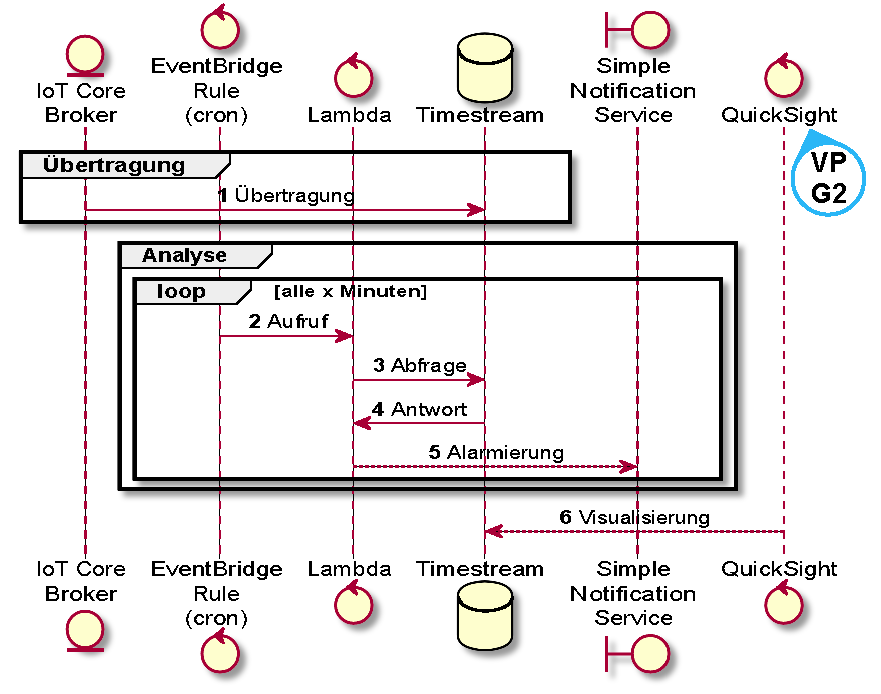
\includegraphics[width=\textwidth]{graphics/batch-ra.pdf}
\caption{Sequenzdiagramm Batch Verarbeitung}
\label{abb:SequenceBatchRA}
\end{figure}

\subsection{Verteilungssicht}
\begin{figure}[H]
\centering
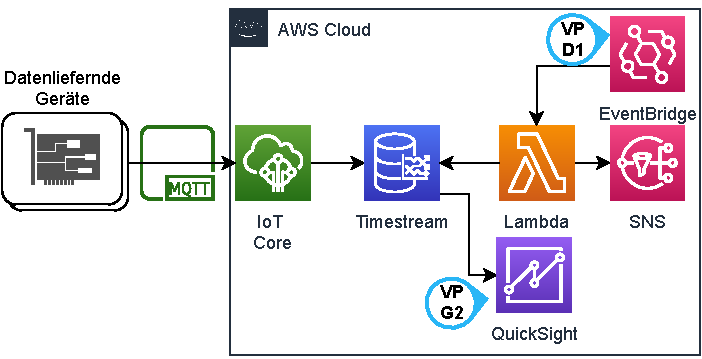
\includegraphics[width=\textwidth]{graphics/DB-RA-Overview.pdf}
\caption{Top Level View Referenzarchitektur}
\label{abb:TopLevelDBRA}
\end{figure}

Variationspunkt 1: Hier wird eine Dashboardinglösung, im speziellen der \ac{AWS} eigenen Dienst QuickSight eingeplant. \TodoW{Warum nicht CloudWatch (P)} Dies erfolgt, damit Benachrichtigungen, die via \ac{SNS} versendet werden, leicht für die Benachrichtigten nachvollziehbar sind. Wenn also beispielsweise eine Anomalie erkannt wurde, kann dies mit einer Visualisierung nachvollzogen werden, um dann entsprechend zu handeln. Wichtig ist, dass die Visualisierung sowohl von den Originaldaten aus dem Speicher von \AWSIOT{} Analytics gespeist wird, als auch aus der Analyse. Eine Visualisierung sieht wie folgt aus:

\begin{figure}[H]
\centering
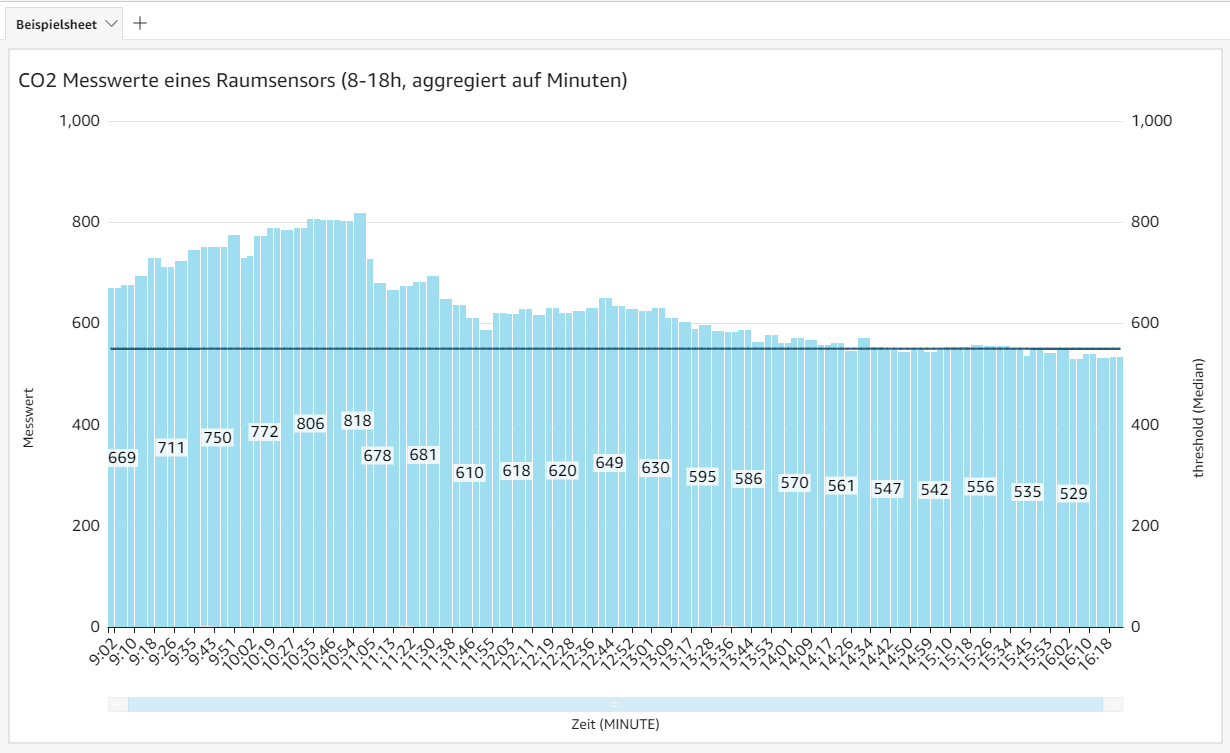
\includegraphics[width=\textwidth]{graphics/QuickSight-Beispiel.png}
\caption{Dashboard in Quicksight}
\label{abb:DashboardDBRA}
\end{figure}

Hier können Benachrichtigte direkt ablesen, dass ständige Schwellwert-Alarme am Morgen ihre Berechtigung hatten, da der Schwellwert erst gegen 14.30 Uhr unterschritten wurde. Entsprechend Maßnahmen, wie beispielsweise die gezielte Belüftung des Raums, in welchem dieser Sensor war, können eingeleitet werden.

\subsection{Bausteinsicht}
\begin{figure}[H]
\centering
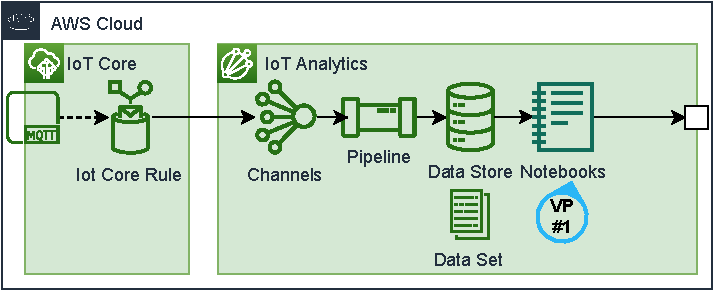
\includegraphics[width=\textwidth]{graphics/DB-RA-Elements.pdf}
\caption{Interagierende Dienstelemente}
\label{abb:ElementeDBRA}
\end{figure}

\subsection{Anforderungen}
\begin{itemize}
\item Anwendbarkeit auf Monitoring (klassische IT)
\item Anwendbarkeit auf Sensordaten (\ac{IoT})
\item Wertschöpfung für den Betrieb wichtig
\item akzeptabel und problemlösend für Domäne
\item Handling von Events, Messwerten und \enquote{Streaming}
\item automatisierte operative Entscheidungen
\end{itemize}

\subsection{Operations}

\begin{table}[H]
\centering
\begin{tabular}{|l|l|l|l|}
\hline
Dienst & Metrik & Ursache & Detektionsart \\ \hline
\rowcolor[HTML]{F5F5F5} 
\ac{SNS} & NumberOfNotificationsFailed & Dienstfehler & Schwellwert \\ \hline

\multirow{2}{*}{\AWSIOT{} Core} & RuleMessageThrottled & \begin{tabular}[c]{@{}l@{}}Dienstfehler/\\ Benutzungsfehler\end{tabular} & Schwellwert \\ \cline{2-4} 
 & Failure & \begin{tabular}[c]{@{}l@{}}Dienstfehler/\\ Benutzungsfehler\end{tabular} & Schwellwert \\ \hline
 
\rowcolor[HTML]{F5F5F5} 
\cellcolor[HTML]{F5F5F5} & SystemErrors & Dienstfehler & Schwellwert \\ \cline{2-4} 
\rowcolor[HTML]{F5F5F5} 
\cellcolor[HTML]{F5F5F5} & UserErrors & Benutzungsfehler & Schwellwert \\ \cline{2-4} 
\rowcolor[HTML]{F5F5F5} 
\multirow{-3}{*}{\cellcolor[HTML]{F5F5F5}TimeStream} & SuccessfulRequestLatency & \begin{tabular}[c]{@{}l@{}}Dienstfehler/\\ Benutzungsfehler\end{tabular} & Anomalie \\ \hline

\multirow{3}{*}{Lambda} & Duration & \begin{tabular}[c]{@{}l@{}}Dienstfehler/\\ Benutzungsfehler\end{tabular} & Anomalie \\ \cline{2-4} 
 & Errors & \begin{tabular}[c]{@{}l@{}}Dienstfehler/\\ Benutzungsfehler\end{tabular} & Schwellwert \\ \cline{2-4} 
 & Throttles & Benutzungsfehler & Schwellwert \\ \hline
\end{tabular}
\caption{CloudWatch Metriken}
\label{tab:cloudwatch-metrics-db}
\end{table}


TimeStream \footcite[Vgl.][]{AmazonWebServicesInc..o.J.be}
Lambda \footcite[Vgl.][]{AmazonWebServicesInc..o.J.bf}
\ac{SNS} \footcite[Vgl.][]{AmazonWebServicesInc..o.J.bc}
\AWSIOT{} Core \footcite[Vgl.][]{AmazonWebServicesInc..o.J.az}

\subsection{Know-how}


\section{Einsatzszenarien der Referenzmodelle}


Chaos Engineering nicht vergessen \footcite[Vgl.][]{Augsten.2020}

Innerhalb dieser Arbeit wurden Referenzarchitekturen für die Verarbeitung in der Cloud konstruiert. Ein Trend, der dabei ausgespart wurde, ist das sogenannte \enquote{Fog computing}. Nach der Definition von \citeauthor{Vaquero.2014} ist Fog computing ein Szenario, in dem heterogene, allgegenwärtige und dezentralisierte Geräte kommunizieren und kooperieren um Speicher- und Verarbeitungsaufgaben zu übernehmen.\footcite[Vgl.][30\psq]{Vaquero.2014} In der Praxis führt dies dazu, dass Verarbeitungsaufgaben in Teilen, angelehnt an das \enquote{Edge computing} von der Cloud in Richtung der Geräte ausgelagert wird.\footcite[Vgl.][]{Bonomi.2012} Dies geschieht dabei beispielsweise an Netzwerkgateways, die sowieso mit der Cloud kommunizieren und folgend nur noch bereits ausgewertete Daten übertragen.